% Canonical LaTeX edition. The original Typst edition is retained separately.
% Compile with: tectonic sidewalkpilot-5C-math-and-cs.tex
\documentclass[11pt,letterpaper]{article}
\usepackage[margin=0.68in,headheight=13pt,headsep=14pt,footskip=25pt]{geometry}
\usepackage[OT1]{fontenc}
\renewcommand{\rmdefault}{cmr}
\renewcommand{\sfdefault}{cmss}
\renewcommand{\ttdefault}{cmtt}
\usepackage{amsmath,amssymb}
\usepackage{tikz}
\usetikzlibrary{arrows.meta}
\usepackage{xcolor,booktabs,tabularx,array,enumitem,fancyhdr,titlesec,listings}
\usepackage[hidelinks]{hyperref}
% No replacement text or math font: retain the classic Computer Modern family.
\definecolor{ink}{HTML}{193B38}
\definecolor{blue}{HTML}{235B83}
\definecolor{muted}{HTML}{57616B}
\definecolor{pale}{HTML}{EDF4F3}
\definecolor{codebg}{HTML}{F2F4F6}
\definecolor{accent}{HTML}{A34228}
\tikzset{unit/.style={circle,draw=ink,thick,minimum size=11mm,inner sep=2pt},
 block/.style={draw=ink,thick,minimum height=10mm,align=center,inner sep=5pt},
 flow/.style={-{Stealth[length=2.5mm]},thick,draw=ink},
 grad/.style={-{Stealth[length=2.5mm]},thick,dashed,draw=accent}}
\hypersetup{pdftitle={SidewalkPilot 5.C: Mathematics and Computer Science},
 pdfauthor={SidewalkPilot project; AI-assisted technical guide}}
\pagestyle{fancy}
\fancyhf{}
\fancyhead[L]{\scriptsize\sffamily\color{muted}SIDEWALKPILOT / 5.C / IMPLEMENTATION GUIDE}
\fancyfoot[R]{\scriptsize\sffamily\color{muted}22 NOV 2026\quad\thepage}
\renewcommand{\headrulewidth}{0pt}
\setlength{\parindent}{0pt}
\setlength{\parskip}{5pt}
\setlength{\emergencystretch}{2em}
\raggedbottom
\titleformat{\section}{\sffamily\bfseries\color{ink}\fontsize{21}{24}\selectfont}{}{0pt}{}
\titleformat{\subsection}{\sffamily\bfseries\color{blue}\large}{}{0pt}{}
\titlespacing*{\section}{0pt}{0pt}{7pt}
\titlespacing*{\subsection}{0pt}{10pt}{3pt}
\setlist{nosep,leftmargin=1.4em,topsep=4pt}
\setlength{\tabcolsep}{5pt}
\renewcommand{\arraystretch}{1.12}
\newcolumntype{Y}{>{\raggedright\arraybackslash}X}
\newcommand{\code}[1]{\texttt{\detokenize{#1}}}
\newcommand{\note}[1]{\par\vspace{3pt}\begingroup\setlength{\fboxsep}{8pt}%
 \colorbox{pale}{\parbox{\dimexpr\linewidth-2\fboxsep\relax}{#1}}\endgroup\par\vspace{3pt}}
\newcommand{\guidepage}[2]{\clearpage\pdfbookmark[0]{#1}{guide-\thepage}\section*{#1}{\sffamily\color{muted}#2}\par\vspace{5pt}}
\newcommand{\op}[1]{\operatorname{#1}}
\newcommand{\refsource}[2]{\href{#1}{\textcolor{blue}{#2}}}
\lstset{language=Python,basicstyle=\ttfamily\footnotesize,
 keywordstyle=\color{blue},commentstyle=\color{muted},stringstyle=\color{ink},
 backgroundcolor=\color{codebg},frame=none,breaklines=true,columns=fullflexible,
 keepspaces=true,showstringspaces=false,xleftmargin=6pt,xrightmargin=6pt,
 aboveskip=7pt,belowskip=6pt}
\begin{document}
\setlength{\abovedisplayskip}{6pt}
\setlength{\belowdisplayskip}{6pt}
\setlength{\abovedisplayshortskip}{3pt}
\setlength{\belowdisplayshortskip}{4pt}
{\small\sffamily\bfseries\color{muted}MATHEMATICS + COMPUTER SCIENCE}
\vspace{8pt}
\pdfbookmark[0]{SidewalkPilot 5.C}{guide-title}
\section*{SidewalkPilot 5.C}
{\sffamily\large\color{blue}How the segmentation model actually works}

\textbf{ConvNeXt-Tiny encoder + custom U-Net-style decoder. Full FP32.}

This guide follows the code in the current \code{series-5} checkout. It explains what happens to an image, how a mask is predicted, how training changes weights, and what changes when the same network runs normally. Equations describe the implemented model, not a different architecture we might build later.

\note{\textbf{The central distinction:} inference computes a prediction using existing weights. Training computes a prediction, compares it with a target, differentiates the error, and updates those weights. A forward pass alone does not teach the model anything.}

\subsection*{The two paths}
\textbf{Training}
\[
\text{image + target}\to\text{prediction}\to\text{loss}\to\text{gradients}\to\text{updated weights}
\]
\textbf{Normal inference}
\[
\text{image}\to\text{fixed trained weights}\to\text{sidewalk/background mask}
\]
\subsection*{What is fixed for this version?}
\begin{tabularx}{\linewidth}{@{}lY@{}}\toprule
Model name & \textbf{5.C}, an uppercase-letter beta\\
Model input & 960 wide by 540 high; RGB; FP32\\
Model output & Two scores per pixel: background and sidewalk\\
Encoder / decoder & ConvNeXt-Tiny / three skip-fusion stages\\
Trainable parameters & 28,855,298 (about 28.9 million)\\
Initialization & ImageNet encoder; newly initialized decoder\\
Default batch / limit & 8 images / 20 epochs, with early stopping\\\bottomrule
\end{tabularx}
\subsection*{Reading map}
Start on page 2: every part of image normalization is unpacked before the architecture. Then follow the small weight/bias examples into tensors, convolution, the encoder/decoder, loss, and learning. The final pages cover inference, evaluation, source code, and a symbol dictionary. PDF bookmarks follow the section headings.

The diagrams use original examples and are drawn directly in LaTeX. They build intuition with small numbers; they are not copied book illustrations or visualizations of learned 5.C weights. Small teaching networks are explicitly distinguished from the implemented model.

{\small\textbf{Status:} architecture and numerical checks are implemented. A short setup smoke test is not a completed 5.C experiment. This document does not launch training, claim final accuracy, or establish real-time Jetson performance. The data campaign and release still require quality checks.}

\guidepage{1. Meet mu and sigma}{Read the normalization equation one symbol at a time.}
\label{normalization}
\[
\boxed{x_{c,h,w}=\frac{I_{c,h,w}/255-\mu_c}{\sigma_c}}
\]
\textbf{Say it aloud:} take one color value, divide it by 255, subtract that color channel's reference mean, and divide by that channel's reference standard deviation. The result is the number the model receives at that position.

\begin{tabularx}{\linewidth}{@{}lY@{}}\toprule
\textbf{Symbol} & \textbf{Meaning here}\\\midrule
$I_{c,h,w}$ & One RGB value in the resized image, before normalization. For an 8-bit color channel its range is 0 to 255.\\
$c,h,w$ & Indices: which color channel, which row, which column. A subscript selects an entry; it is not multiplication.\\
$\mu_c$ & Lowercase Greek \textbf{mu}, pronounced ``mew'': the reference \textbf{mean} for channel $c$, on the 0-to-1 scale. A mean describes the center.\\
$\sigma_c$ & Lowercase Greek \textbf{sigma}, pronounced ``SIG-muh'': the reference \textbf{standard deviation}. It describes spread, in the same units as the 0-to-1 values.\\
$x_{c,h,w}$ & The normalized value: its signed distance from the reference center, measured in reference standard deviations.\\\bottomrule
\end{tabularx}

\subsection*{Three channels, three pairs of constants}
\[
\begin{array}{c|ccc}
 &\text{red}&\text{green}&\text{blue}\\\hline
\mu_c&0.485&0.456&0.406\\
\sigma_c&0.229&0.224&0.225
\end{array}
\]
These are fixed preprocessing constants used with the ImageNet-pretrained encoder. They are \textbf{not learned weights}, not recalculated from each sidewalk image, and not estimated from the held-out test set. The same transform is used for training and normal prediction. [C3, R9]

\subsection*{Follow an actual red-channel value}
\begin{center}
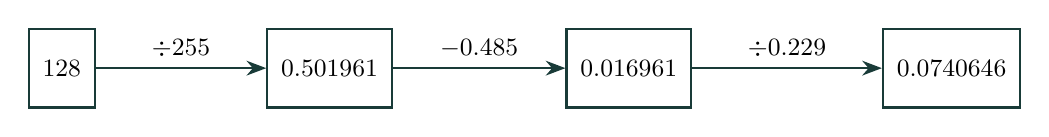
\begin{tikzpicture}[font=\small]
\node[block] (a) at (0,0) {$128$};
\node[block] (b) at (3.4,0) {$0.501961$};
\node[block] (c) at (7.2,0) {$0.016961$};
\node[block] (d) at (11.3,0) {$0.0740646$};
\draw[flow] (a)--node[above] {$\div255$}(b);
\draw[flow] (b)--node[above] {$-0.485$}(c);
\draw[flow] (c)--node[above] {$\div0.229$}(d);
\end{tikzpicture}
\end{center}
The red value is only about $0.074$ reference standard deviations above the reference mean. A negative result would mean \emph{below} the mean, not a negative light intensity or an error. Values outside $[0,1]$ are expected after normalization.

\note{Why do this? The pretrained encoder learned using a particular input scale. Keeping that scale avoids an unnecessary preprocessing mismatch. It does not make every image's mean zero, guarantee better masks, or change which pixels the target labels call sidewalk.}

\guidepage{2. Mean, variance, and spread}{Where the ideas behind mu and sigma come from.}
\subsection*{An arithmetic mean is a center}
Use four made-up channel values, already scaled to $[0,1]$: $q_1=0.1$, $q_2=0.3$, $q_3=0.5$, $q_4=0.7$. If $M$ is the number of values,
\[
\mu=\frac{1}{M}\sum_{j=1}^{M}q_j
=\frac{0.1+0.3+0.5+0.7}{4}=0.4.
\]
The large $\sum$ is \textbf{capital sigma}, a summation sign: ``add the terms as $j$ runs from 1 to $M$.'' It is not the lowercase $\sigma$ used for standard deviation.

\subsection*{Why square the distances?}
The signed distances from the mean are $-0.3,-0.1,0.1,0.3$. Their sum is zero even though the values are spread out. Squaring keeps the distances from canceling:
\[
v=\frac{1}{M}\sum_{j=1}^{M}(q_j-\mu)^2
=\frac{0.09+0.01+0.01+0.09}{4}=0.05.
\]
$v$ is the \textbf{population variance} of these four values. Its units are squared. Taking the positive square root returns to the original units:
\[
\sigma=\sqrt{v}=\sqrt{0.05}\approx0.223607.
\]
This example uses division by $M$. A sample-variance estimator may use $M-1$ for a different statistical purpose. That is not the convention used for the LayerNorm/GroupNorm variance described later.

\begin{center}
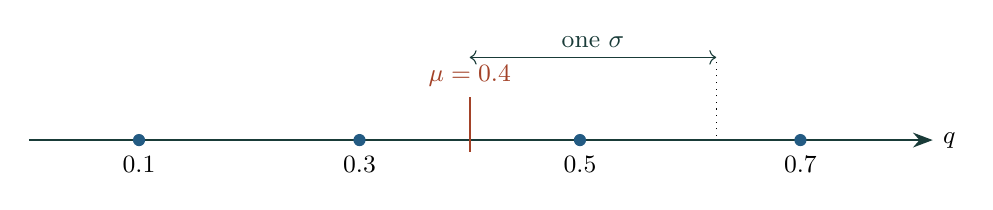
\begin{tikzpicture}[font=\small,x=14cm,y=1cm]
\draw[flow] (0,0)--(.82,0) node[right] {$q$};
\foreach \p in {0.1,0.3,0.5,0.7}{\fill[blue] (\p,0) circle(2.2pt);\node[below] at (\p,-.08){$\p$};}
\draw[accent,thick] (.4,-.15)--(.4,.55) node[above] {$\mu=0.4$};
\draw[<->,ink] (.4,1.05)--(.623607,1.05) node[midway,above] {one $\sigma$};
\draw[dotted] (.623607,.05)--(.623607,1.05);
\end{tikzpicture}
\end{center}

\subsection*{Center, then change the unit of distance}
\begin{tabularx}{\linewidth}{@{}YYYY@{}}\toprule
$q_j$ & $q_j-\mu$ & $\sigma$ & $(q_j-\mu)/\sigma$\\\midrule
0.1 & $-0.3$ & 0.223607 & $-1.34164$\\
0.3 & $-0.1$ & 0.223607 & $-0.44721$\\
0.5 & $0.1$ & 0.223607 & $0.44721$\\
0.7 & $0.3$ & 0.223607 & $1.34164$\\\bottomrule
\end{tabularx}
These four standardized numbers have mean zero and population variance one because we used \emph{their own} mean and variance. SidewalkPilot instead uses fixed ImageNet constants, so its images need not have those statistics after normalization. Dividing by zero would be undefined; the fixed input $\sigma_c$ values are positive, while internal normalization adds a small $\epsilon$ for stability.

\guidepage{3. One neuron: weights and bias}{Multiplication controls each input; addition shifts the total.}
\[
z=w_1x_1+w_2x_2+b.
\]
$x_1,x_2$ are two input numbers. $w_1,w_2$ are two learned \textbf{weights}. $b$ is a learned \textbf{bias}, added once after the products are summed. $z$ is the resulting score, called a pre-activation when an activation function follows it.

\begin{center}
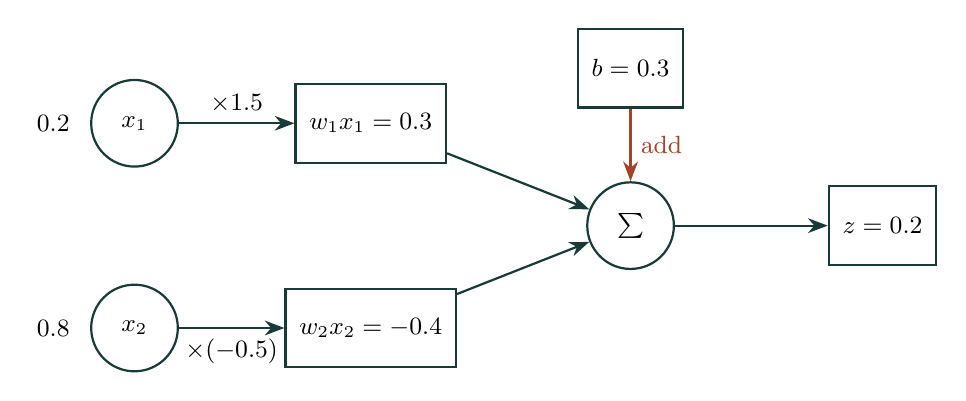
\begin{tikzpicture}[font=\small]
\node[unit] (x1) at (0,1.3) {$x_1$};
\node[left] at (-.7,1.3) {$0.2$};
\node[unit] (x2) at (0,-1.3) {$x_2$};
\node[left] at (-.7,-1.3) {$0.8$};
\node[block] (p1) at (3,1.3) {$w_1x_1=0.3$};
\node[block] (p2) at (3,-1.3) {$w_2x_2=-0.4$};
\node[unit] (sum) at (6.3,0) {$\sum$};
\node[block] (bias) at (6.3,2) {$b=0.3$};
\node[block] (out) at (9.5,0) {$z=0.2$};
\draw[flow] (x1)--node[above] {$\times1.5$}(p1);
\draw[flow] (x2)--node[below] {$\times(-0.5)$}(p2);
\draw[flow] (p1)--(sum);\draw[flow] (p2)--(sum);
\draw[flow,accent] (bias)--node[right] {add}(sum);
\draw[flow] (sum)--(out);
\end{tikzpicture}
\end{center}
\[
z=\underbrace{1.5\times0.2}_{0.3}
+\underbrace{(-0.5)\times0.8}_{-0.4}+0.3=0.2.
\]
\textbf{Positive weight:} increasing that input increases $z$, holding everything else fixed. \textbf{Negative weight:} increasing that input decreases $z$. \textbf{Zero weight:} that input has no direct effect through this connection. A larger magnitude means a stronger effect per unit change in the input.

\subsection*{Bias is not another measured feature}
With both inputs zero, $z=b$. Bias therefore lets a unit have a nonzero starting offset. Equivalently, imagine an extra constant input $x_0=1$ and a weight $w_0=b$: its contribution is always $b\times1$. Here ``bias'' means an additive parameter, not unfairness in data or an error in an experiment.

\subsection*{Where is the activation?}
A hidden unit may then compute $a=f(z)$, where $f$ is an activation function. ConvNeXt and the decoder's fusion blocks use \textbf{GELU}. The final class head instead produces logits with no GELU after that head. The diagram isolates the weighted sum; it is not the whole 5.C model.

\note{Inputs and activations change with each image. Weights and biases are stored model parameters shared across predictions. Training changes them through gradients; ordinary inference reads them without updating them.}

\guidepage{4. See what a weight or bias changes}{The two parameters do different geometric jobs.}
For one input, $z=wx+b$ is a line. The horizontal axis is the input $x$ and the vertical axis is the output score $z$. A score is not yet a probability.

\begin{center}
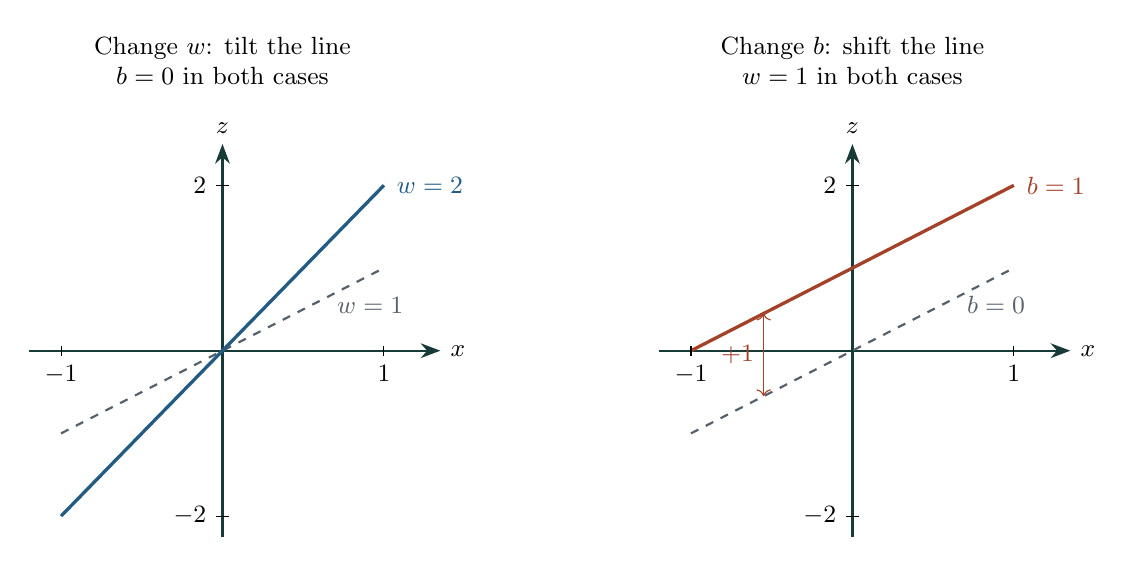
\begin{tikzpicture}[font=\small]
\begin{scope}[x=2.05cm,y=1.05cm]
\draw[flow] (-1.2,0)--(1.35,0) node[right] {$x$};
\draw[flow] (0,-2.25)--(0,2.5) node[above] {$z$};
\draw[muted,dashed,thick] (-1,-1)--(1,1);
\draw[blue,very thick] (-1,-2)--(1,2);
\node[above,align=center] at (0,3.1) {Change $w$: tilt the line\\$b=0$ in both cases};
\node[right,blue] at (1.02,2) {$w=2$};
\node[right,muted] at (.65,.55) {$w=1$};
\foreach \x in {-1,1}{\draw (\x,.06)--(\x,-.06) node[below] {$\x$};}
\foreach \z in {-2,2}{\draw (.04,\z)--(-.04,\z) node[left] {$\z$};}
\end{scope}
\begin{scope}[shift={(8,0)},x=2.05cm,y=1.05cm]
\draw[flow] (-1.2,0)--(1.35,0) node[right] {$x$};
\draw[flow] (0,-2.25)--(0,2.5) node[above] {$z$};
\draw[muted,dashed,thick] (-1,-1)--(1,1);
\draw[accent,very thick] (-1,0)--(1,2);
\node[above,align=center] at (0,3.1) {Change $b$: shift the line\\$w=1$ in both cases};
\node[right,accent] at (1.02,2) {$b=1$};
\node[right,muted] at (.65,.55) {$b=0$};
\draw[<->,accent] (-.55,-.55)--(-.55,.45) node[midway,left] {$+1$};
\foreach \x in {-1,1}{\draw (\x,.06)--(\x,-.06) node[below] {$\x$};}
\foreach \z in {-2,2}{\draw (.04,\z)--(-.04,\z) node[left] {$\z$};}
\end{scope}
\end{tikzpicture}
\end{center}
\subsection*{Read the diagrams numerically}
At $x=0.5$, changing $w$ from 1 to 2 with $b=0$ changes $z$ from 0.5 to 1. Changing $b$ from 0 to 1 with $w=1$ changes $z$ from 0.5 to 1.5. Bias shifts the line by the same amount at every input; changing a weight does not.

\subsection*{A threshold gives a decision boundary}
In a simplified two-class model with logits $(0,z)$, sidewalk is favored when $z>0$. If $w\ne0$, the boundary is
\[
wx+b=0\quad\Longrightarrow\quad x=-\frac{b}{w}.
\]
With two inputs, $w_1x_1+w_2x_2+b=0$ describes a line in the input plane. Weights set its direction; bias shifts its position. A network stacks these transformations with nonlinearities, allowing much more complicated boundaries than one straight line.

\note{This is a geometric teaching example. 5.C uses many learned feature channels and convolutional operations; its sidewalk boundary in a photograph is not this one-dimensional threshold. At equal logits, the implementation's argmax selects class 0, so equality is not a positive sidewalk decision.}

\guidepage{5. From one neuron to a layer}{A matrix is a compact way to write many weighted sums.}
A \textbf{vector} is an ordered list of numbers. A \textbf{matrix} is a rectangular array. Let $x$ contain two inputs, $W$ contain two rows of weights, and $b$ contain one bias per output:
\[
\underbrace{\begin{bmatrix}z_1\\z_2\end{bmatrix}}_{z}
=\underbrace{\begin{bmatrix}1.5&-0.5\\-0.5&1\end{bmatrix}}_{W}
\underbrace{\begin{bmatrix}0.2\\0.8\end{bmatrix}}_{x}
+\underbrace{\begin{bmatrix}0.3\\-0.1\end{bmatrix}}_{b}
=\begin{bmatrix}0.2\\0.6\end{bmatrix}.
\]
Each output uses \textbf{one row} of $W$. The first row gives $1.5(0.2)-0.5(0.8)+0.3=0.2$. The second gives $-0.5(0.2)+1(0.8)-0.1=0.6$. Here 1 and 2 number outputs, not dataset class IDs.

\begin{center}
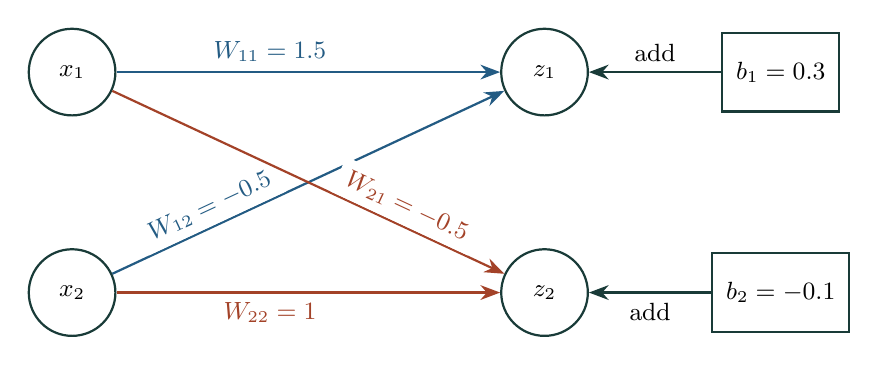
\begin{tikzpicture}[font=\small]
\node[unit] (x1) at (0,1.4) {$x_1$};
\node[unit] (x2) at (0,-1.4) {$x_2$};
\node[unit] (z1) at (6,1.4) {$z_1$};
\node[unit] (z2) at (6,-1.4) {$z_2$};
\draw[flow,blue] (x1)--node[pos=.4,above] {$W_{11}=1.5$}(z1);
\draw[flow,blue] (x2)--node[pos=.27,above,sloped,fill=white] {$W_{12}=-0.5$}(z1);
\draw[flow,accent] (x1)--node[pos=.73,above,sloped,fill=white] {$W_{21}=-0.5$}(z2);
\draw[flow,accent] (x2)--node[pos=.4,below] {$W_{22}=1$}(z2);
\node[block] (b1) at (9,1.4) {$b_1=0.3$};
\node[block] (b2) at (9,-1.4) {$b_2=-0.1$};
\draw[flow] (b1)--node[above]{add}(z1);
\draw[flow] (b2)--node[below]{add}(z2);
\end{tikzpicture}
\end{center}
\subsection*{Count the parameters, not the arrows in a drawing}
There are four weights plus two biases: six trainable numbers. In general, a dense layer with $C_{\rm in}$ inputs and $C_{\rm out}$ outputs has $C_{\rm out}C_{\rm in}$ weights and, when enabled, $C_{\rm out}$ biases. The symbol $W_{o,c}$ selects the weight from input $c$ to output $o$.

\subsection*{How this connects to the real mask head}
At each position in the decoder's $135\times240$ feature map, 5.C's $1\times1$ head takes a vector of \textbf{32 features} and computes \textbf{2 logits}. Its weight shape is \code{[2, 32, 1, 1]}, with two biases: $2(32)+2=66$ parameters. Those same 66 parameters are reused at every spatial position, not copied into separate learned values per pixel. [C1]

\note{A convolution's $1\times1$ label describes its spatial footprint. It can still mix many input channels. One output score is a sum across channels, not just multiplication of one image pixel by one number.}

\guidepage{6. The tensor map}{An image becomes feature maps, then a mask.}
\subsection*{Mathematics view}
A tensor is a multidimensional array. PyTorch image batches use $[N,C,H,W]$: batch size, channels, height, width. A feature channel is a learned response map, not a manually assigned object class. Here $N=8$ during default training and usually $N=1$ during inference.

{\small
\begin{tabularx}{\linewidth}{@{}YY Y@{}}\toprule
\textbf{Operation} & \textbf{Output: $C\times H\times W$} & \textbf{Role}\\\midrule
RGB input & $3\times540\times960$ & Normalized image\\
Stem: $4\times4$, stride 4 & $96\times135\times240$ & Initial features\\
Stage 1: 3 blocks & $96\times135\times240$ & Skip $E_1$\\
Downsample + stage 2 & $192\times67\times120$ & 3 blocks; skip $E_2$\\
Downsample + stage 3 & $384\times33\times60$ & 9 blocks; skip $E_3$\\
Downsample + stage 4 & $768\times16\times30$ & 3 blocks; deepest $E_4$\\
Bottleneck projection & $256\times16\times30$ & Decoder input\\
Fuse with $E_3$ & $128\times33\times60$ & Decoder \code{up16}\\
Fuse with $E_2$ & $64\times67\times120$ & Decoder \code{up8}\\
Fuse with $E_1$ & $32\times135\times240$ & Decoder \code{up4}\\
$1\times1$ classifier & $2\times135\times240$ & Two class logits\\
Bilinear resize & $2\times540\times960$ & Model return value\\\bottomrule
\end{tabularx}}

\subsection*{Computer science view}
The encoder saves four outputs from \code{features[1]}, \code{[3]}, \code{[5]}, and \code{[7]}. The decoder takes these in order from deepest to shallowest. \code{model(image)["out"]} returns a floating-point tensor, \textbf{not} a colored PNG or a list of steering commands.

The heights are deliberately \textbf{135, 67, 33, 16}, not rounded-up multiples. Unpadded stride-2 downsampling takes the floor. The decoder resizes to each skip's exact dimensions, so odd-sized feature maps still align.

\note{\textbf{Width versus height:} we say $960\times540$ for a picture, but write \code{[N, 3, 540, 960]} in code. Existing $1280\times720$ dataset images are resized for the network; the model's input size is not a claim about the camera's active capture configuration.}
\[
\begin{array}{ccccccc}
E_1:96&\to&E_2:192&\to&E_3:384&\to&E_4:768\\
\downarrow\text{skip}&&\downarrow\text{skip}&&\downarrow\text{skip}&&\downarrow\text{project}\\
D_1:32&\leftarrow&D_2:64&\leftarrow&D_3:128&\leftarrow&D_4:256
\end{array}
\]
{\small Encoder flows right; decoder flows left. Numbers are channels. $D_1$ feeds the class head and output resize. Skips are projected and concatenated, not simply added. The accompanying shape capture verifies the listed shapes and dtypes. [C1, C2]}

\guidepage{7. Pixels and convolution}{How numerical image features are made.}
\subsection*{Input preparation}
Images are converted to RGB, resized to $960\times540$ with bilinear interpolation, converted from bytes to FP32 values in $[0,1]$, then normalized channel by channel:
\[
x_{c,h,w}=\frac{I_{c,h,w}/255-\mu_c}{\sigma_c},
\qquad \mu=(0.485,0.456,0.406),\quad \sigma=(0.229,0.224,0.225).
\]
These are the normalization constants used with the ImageNet initialization. For example, a red value of 128 becomes approximately
\[
\frac{128/255-0.485}{0.229}\approx0.074.
\]
Values after normalization can be negative or above one. That is expected.

\subsection*{What a convolution calculates}
For dilation 1, a convolution output is a weighted sum over an image patch and its input channels:
\[
Y_{o,h,w}=b_o+\sum_{c,u,v} K_{o,c,u,v}\,X_{c,sh+u-p,sw+v-p}.
\]
Here $o$ selects an output channel and $c$ an input channel; $h,w$ select the output position, while $u,v$ run over the kernel's rows and columns. $\sum_{c,u,v}$ means add over all input channels and all kernel positions. $K$ contains learned weights, $b_o$ is an optional output-channel bias, $s$ is stride (the step between patches), and $p$ is zero-padding width. PyTorch applies the kernel without flipping it, technically cross-correlation. For kernel width $k$ and dilation 1:
\[
H'=\left\lfloor\frac{H+2p-k}{s}\right\rfloor+1.
\]
The floor brackets $\lfloor\ \rfloor$ round down to an integer. $H'$ is output height, not a derivative. For the stem, $k=s=4$, $p=0$, so 540 becomes 135. The first stride-2 downsample turns 135 into 67.

\subsection*{Why learned filters matter}
Early features can respond to local edges, contrast, or texture; later layers combine broader context. These are interpretations of learned representations, not hard-coded promises that a particular channel means ``curb'' or ``shadow.''

A standard convolution has $C_{\mathrm{out}}C_{\mathrm{in}}k^2$ kernel parameters, plus $C_{\mathrm{out}}$ biases when enabled. Its approximate multiply-accumulate count is $H'W'C_{\mathrm{out}}C_{\mathrm{in}}k^2$ per image. Reusing the same kernel at every position is \textbf{weight sharing}.

\subsection*{Computer science view}
The code uses \code{nn.Conv2d}, not Python loops over pixels. PyTorch dispatches tensor operations to CPU or CUDA kernels. Automatic differentiation records enough of the computation to obtain gradients later; the programmer does not hand-write one derivative per weight.

\note{Training labels must \textbf{not} use bilinear resizing: mixing class IDs would create meaningless labels. Training masks use nearest-neighbor resizing; images and class scores may use bilinear resizing. [C3]}

\guidepage{8. A convolution you can calculate}{Nine products, one sum, one bias; then reuse the weights.}
Consider a single-channel $3\times3$ patch $X$ and kernel $K$. These deliberately small numbers are a teaching example, not the trained model's actual filter.
\[
X=\begin{bmatrix}1&2&0\\0&1&3\\2&0&1\end{bmatrix},\qquad
K=\begin{bmatrix}1&0&-1\\1&0&-1\\1&0&-1\end{bmatrix},\qquad b=0.5.
\]
\begin{center}
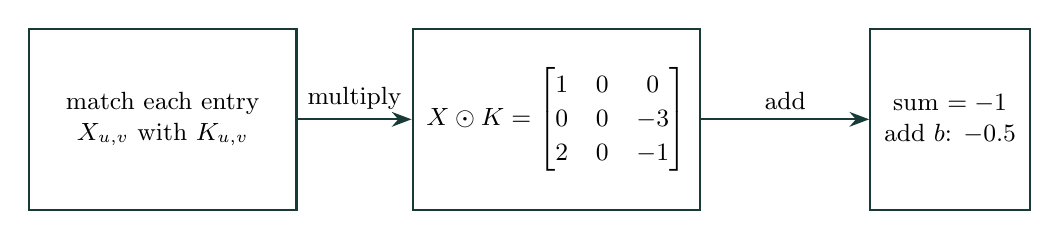
\begin{tikzpicture}[font=\small]
\node[block,minimum width=34mm,minimum height=23mm] (x) at (0,0)
 {match each entry\\$X_{u,v}$ with $K_{u,v}$};
\node[block,minimum height=23mm] (p) at (5,0)
 {$X\odot K=\begin{bmatrix}1&0&0\\0&0&-3\\2&0&-1\end{bmatrix}$};
\node[block,minimum height=23mm] (z) at (10,0) {sum $=-1$\\add $b$: $-0.5$};
\draw[flow] (x)--node[above]{multiply}(p);
\draw[flow] (p)--node[above]{add}(z);
\end{tikzpicture}
\end{center}
\[
Y=1+0+0+0+0-3+2+0-1+0.5=-0.5.
\]
$\odot$ denotes elementwise multiplication: multiply entries in the same position. It is different from matrix multiplication, which forms row-by-column sums. A negative filter response is allowed; a later activation may transform it.

\subsection*{Slide the kernel, not its parameter values}
\begin{center}
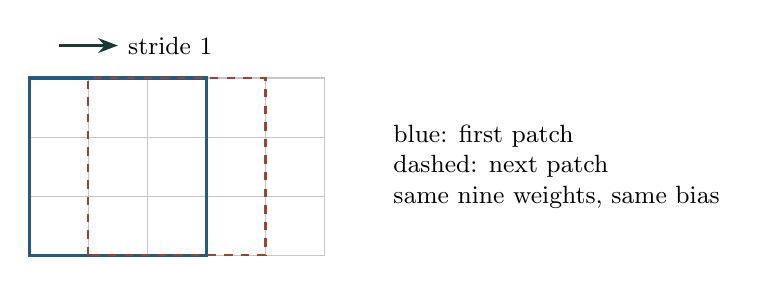
\begin{tikzpicture}[font=\small,x=.75cm,y=.75cm]
\draw[step=1,gray!45] (0,0) grid (5,3);
\draw[blue,very thick] (0,0) rectangle (3,3);
\draw[accent,thick,dashed] (1,0) rectangle (4,3);
\draw[flow] (.5,3.55)--(1.5,3.55) node[right] {stride 1};
\node[align=left,anchor=west] at (6,1.5)
 {blue: first patch\\dashed: next patch\\same nine weights, same bias};
\end{tikzpicture}
\end{center}
A new patch changes the products, not the kernel's stored numbers. Training receives gradient contributions from every location that used each weight. At inference the kernel stays fixed while it scans all positions.

\subsection*{Extend this to the real network}
With 32 input channels, one $3\times3$ output filter has $32\times9=288$ weights, not nine. It sums over all 32 channel patches before adding its one bias, if enabled. With 64 output channels, there are 64 such filters.

The 5.C decoder's fusion convolutions use \code{bias=False}; GroupNorm supplies a learned affine offset afterward. The bottleneck, skip projections, and class head \emph{do} have biases. A $1\times1$ head uses one spatial position but still sums across channels. Interpolation has numerical blending coefficients, but they are not learned parameters. [C1]

\guidepage{9. Inside ConvNeXt}{Tiny describes a model size, not the quality of its predictions.}
\subsection*{The residual block}
The four stages contain 3, 3, 9, and 3 blocks, at 96, 192, 384, and 768 channels. Within each block, with input $X$:
\begin{align*}
U&=\op{DWConv}_{7\times7}(X),\\
V&=\op{LN}(U),\qquad A=W_1V+b_1,\qquad B=\op{GELU}(A),\\
R&=W_2B+b_2,\qquad Y=X+\op{DropPath}(\gamma\odot R).
\end{align*}
These channel-mixing equations apply independently at every spatial location. $W_1$ expands $C$ channels to $4C$; $W_2$ reduces them back to $C$. The learned scale $\gamma$ has one value per channel; $\odot$ means elementwise scaling. The input and residual have equal shapes, so they can be added. [R1, R2]

\subsection*{What each operation does}
\textbf{Depthwise convolution:} each channel gets its own $7\times7$ spatial kernel (\code{groups=C}). It uses $49C$ kernel parameters rather than $49C^2$ for a dense same-width convolution. Channel mixing happens in the later linear layers.

\textbf{Layer normalization:} at each spatial position, normalize across channels:
\[
\op{LN}(u_c)=a_c\frac{u_c-\bar{u}}{\sqrt{v+\epsilon}}+b_c.
\]
$\bar{u}$ and $v$ are that position's channel mean and population variance. $a_c,b_c$ are learned affine parameters; $\epsilon=10^{-6}$ prevents division by zero.

\textbf{GELU:} a smooth nonlinear activation $\op{GELU}(a)=a\Phi(a)$, where $\Phi$ is the standard-normal cumulative distribution function. Without nonlinearities, stacking linear operations would have much less expressive power.

\textbf{Residual addition:} the block learns a change to $X$, rather than having to reconstruct all of $X$ from scratch. The identity route also supplies a direct path for gradients.

\subsection*{Computer science view}
Depthwise convolution uses NCHW tensors. The block temporarily permutes to NHWC for channel-wise LayerNorm and \code{nn.Linear}, then permutes back. These are layout changes, not image rotations.

During training, stochastic depth randomly drops a residual branch per sample. Block $j$ uses $p_j=0.1j/17$, for $j=0,\ldots,17$; kept branches are scaled by $1/(1-p_j)$. In evaluation no branch is dropped. Layer scale initializes to $10^{-6}$ in a fresh encoder, but the default pretrained encoder loads its already-learned values.

{\small This encoder is a convolutional network, not a self-attention Transformer. LayerNorm uses the current input in both training and evaluation; it is not BatchNorm with running averages. [C1, R2]}

\guidepage{10. Normalization inside the network}{Same centering idea, different statistics and learned affine parameters.}
Input normalization uses three fixed $\mu_c,\sigma_c$ constants. \textbf{LayerNorm and GroupNorm instead calculate statistics from the current activations}. For the $M$ values in one normalization group,
\[
\bar u=\frac1M\sum_{j=1}^M u_j,\qquad
v=\frac1M\sum_{j=1}^M(u_j-\bar u)^2,\qquad
r_j=\frac{u_j-\bar u}{\sqrt{v+\epsilon}},\qquad y_j=a_jr_j+b_j.
\]
$\bar u$ (``u bar'') is the computed mean. $v$ is the computed population variance. $\epsilon$ (``epsilon'') is a small positive constant inside the square root, so even a zero variance has a nonzero denominator. $a,b$ are learned scale and offset; the computed mean and variance are not optimizer parameters. In GroupNorm, each channel's $a,b$ are shared across spatial positions.

\begin{center}
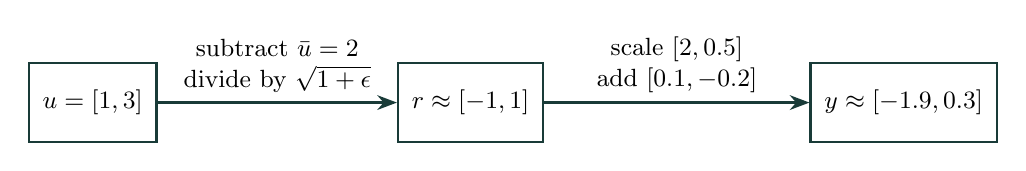
\begin{tikzpicture}[font=\small]
\node[block] (u) at (0,0) {$u=[1,3]$};
\node[block] (r) at (4.8,0) {$r\approx[-1,1]$};
\node[block] (y) at (10.3,0) {$y\approx[-1.9,0.3]$};
\draw[flow] (u)--node[above,align=center]{subtract $\bar u=2$\\divide by $\sqrt{1+\epsilon}$}(r);
\draw[flow] (r)--node[above,align=center]{scale $[2,0.5]$\\add $[0.1,-0.2]$}(y);
\end{tikzpicture}
\end{center}
The values shown are rounded: with $\epsilon>0$ the normalized magnitudes are slightly below one. Learned affine parameters allow the network to choose a useful output scale and offset after standardization.

\begin{tabularx}{\linewidth}{@{}lYY@{}}\toprule
\textbf{Operation} & \textbf{Statistics taken over} & \textbf{What is learned?}\\\midrule
Input transform & Fixed ImageNet RGB reference & Nothing in this transform\\
LayerNorm in a block & All channels at one spatial position, one sample & Scale and bias per channel\\
GroupNorm in decoder & Channels in one of 8 groups, plus all spatial positions, one sample & Scale and bias per channel\\\bottomrule
\end{tabularx}
The encoder uses $\epsilon=10^{-6}$; decoder GroupNorm uses $10^{-5}$. Neither operation uses a running average over earlier batches. Their statistics are computed during both training and evaluation. [C1, R2]

\subsection*{Do not confuse normalization with activation}
Normalization changes centering and scale. An activation introduces a nonlinear relationship. Here GELU is $f(t)=t\Phi(t)$, where $\Phi(t)$ is the probability that a standard-normal random variable is at most $t$. This is a fixed mathematical function, \textbf{not the model's probability of sidewalk}.
\[
f(-1)\approx-0.158655,\qquad f(0)=0,\qquad f(1)\approx0.841345.
\]
GELU smoothly attenuates negative inputs rather than simply deleting them. Normalization and GELU play different roles even when they appear next to each other in code.

\guidepage{11. The U-Net-style decoder}{Context comes up; spatial detail comes across.}
\subsection*{Two different skip connections}
Inside ConvNeXt, a \textbf{residual skip adds} a block's input to its output. Across the encoder and decoder, a \textbf{U-Net-style skip concatenates} a projected encoder feature map with an upsampled decoder map. These are different operations.

Let $E_1,\ldots,E_4$ be the encoder outputs, and $P$ denote a learned $1\times1$ projection. The decoder begins with
\[
D_4=P_4(E_4),\qquad 768\to256\text{ channels}.
\]
Each fusion block then computes
\begin{align*}
T_j&=\op{concat}\bigl(\op{resize}(D_{j+1},\op{size}(E_j)),P_j(E_j)\bigr),\\
D_j&=F_j(T_j),\qquad j=3,2,1.
\end{align*}
$F_j$ is two repetitions of \textbf{$3\times3$ convolution, GroupNorm, GELU}. The final scores are
\[
Z=\op{resize}\bigl(P_{\mathrm{head}}(D_1),(540,960)\bigr).
\]
\begin{tabularx}{\linewidth}{@{}YYYY@{}}\toprule
\textbf{Fusion} & \textbf{Upsampled} & \textbf{Skip projected} & \textbf{Concat / out}\\\midrule
With $E_3$ & 256 channels & 384 to 128 & 384 / 128\\
With $E_2$ & 128 channels & 192 to 64 & 192 / 64\\
With $E_1$ & 64 channels & 96 to 32 & 96 / 32\\\bottomrule
\end{tabularx}

\subsection*{GroupNorm and interpolation}
GroupNorm divides the channels into \textbf{8 groups} per sample and normalizes within each group's channels and spatial positions, with learned per-channel scale and bias. Its epsilon is $10^{-5}$. It does not depend on batch running statistics. [C1]

Bilinear interpolation is a weighted blend of nearby values. With \code{align_corners=False}, an output coordinate $q$ corresponds approximately to $(q+0.5)n_{\mathrm{in}}/n_{\mathrm{out}}-0.5$ in the input, using edge handling at the boundaries. The interpolation itself has no learned weights.

\subsection*{Computer science view}
This is a \textbf{custom, compact U-Net-style decoder}, not an exact reproduction of the original U-Net paper. There are three fusion blocks, no transposed convolutions, and no full-resolution input skip. The two-class head operates at $135\times240$ before logits are enlarged. [C1, R3]

\note{Skip features can help recover boundaries, but upsampling cannot recreate information already lost. More decoder capacity does not automatically fix incorrect labels, missing curb edges, or driveway confusion.}

\guidepage{12. Trace the encoder and decoder}{Follow a real feature map, including the skip connections.}
Each box lists channels $C$ followed by spatial dimensions $H\times W$; the batch axis is omitted. Solid arrows carry the main stream. Dashed arrows carry projected skips. The arrows represent computations, not separate physical processors.
\begin{center}
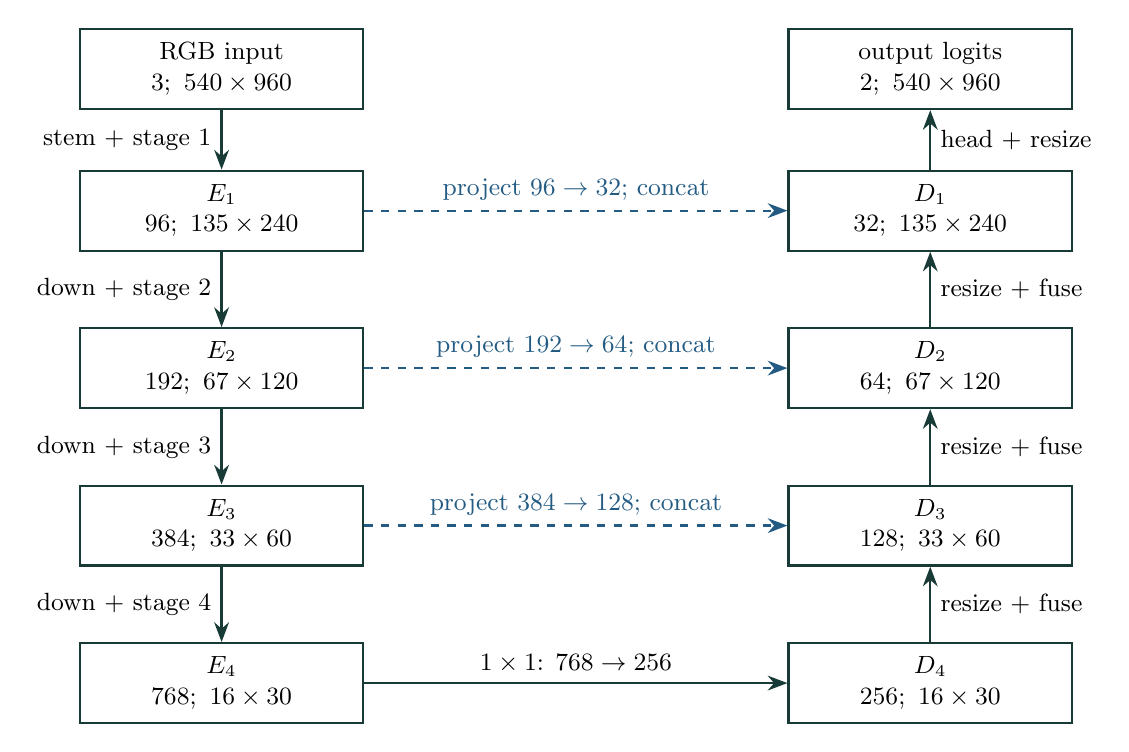
\begin{tikzpicture}[font=\small]
\node[block,minimum width=36mm] (input) at (0,1.5) {RGB input\\$3;\ 540\times960$};
\node[block,minimum width=36mm] (e1) at (0,-.3) {$E_1$\\$96;\ 135\times240$};
\node[block,minimum width=36mm] (e2) at (0,-2.3) {$E_2$\\$192;\ 67\times120$};
\node[block,minimum width=36mm] (e3) at (0,-4.3) {$E_3$\\$384;\ 33\times60$};
\node[block,minimum width=36mm] (e4) at (0,-6.3) {$E_4$\\$768;\ 16\times30$};
\node[block,minimum width=36mm] (d4) at (9,-6.3) {$D_4$\\$256;\ 16\times30$};
\node[block,minimum width=36mm] (d3) at (9,-4.3) {$D_3$\\$128;\ 33\times60$};
\node[block,minimum width=36mm] (d2) at (9,-2.3) {$D_2$\\$64;\ 67\times120$};
\node[block,minimum width=36mm] (d1) at (9,-.3) {$D_1$\\$32;\ 135\times240$};
\node[block,minimum width=36mm] (out) at (9,1.5) {output logits\\$2;\ 540\times960$};
\draw[flow] (input)--node[left]{stem + stage 1}(e1);
\draw[flow] (e1)--node[left]{down + stage 2}(e2);
\draw[flow] (e2)--node[left]{down + stage 3}(e3);
\draw[flow] (e3)--node[left]{down + stage 4}(e4);
\draw[flow] (e4)--node[above]{$1\times1$: $768\to256$}(d4);
\draw[flow] (d4)--node[right]{resize + fuse}(d3);
\draw[flow] (d3)--node[right]{resize + fuse}(d2);
\draw[flow] (d2)--node[right]{resize + fuse}(d1);
\draw[flow] (d1)--node[right]{head + resize}(out);
\draw[flow,dashed,blue] (e3)--node[above]{project $384\to128$; concat}(d3);
\draw[flow,dashed,blue] (e2)--node[above]{project $192\to64$; concat}(d2);
\draw[flow,dashed,blue] (e1)--node[above]{project $96\to32$; concat}(d1);
\end{tikzpicture}
\end{center}
\subsection*{Zoom in on the first fusion}
$D_4$ has 256 channels. Resize its $16\times30$ grid to $33\times60$, matching $E_3$. Separately, a learned $1\times1$ projection changes $E_3$ from 384 to 128 channels. Concatenation stacks the two channel collections: $256+128=384$. Two convolution/GroupNorm/GELU operations reduce and refine this to $D_3$'s 128 channels.

\note{\textbf{Concatenation is not addition.} Concatenating two $C$-channel maps gives $2C$ channels. Adding equally shaped maps gives $C$ channels of sums. ConvNeXt's residual connections add; these encoder-to-decoder connections concatenate.}
The decoder never sees RGB through a full-resolution skip. Its finest feature grid is $135\times240$, so the final interpolation enlarges scores, not newly recovered image detail. The shapes above are checked by real forward hooks. [C1]

\guidepage{13. Weights and FP32}{Architecture, initialization, and precision are separate choices.}
\subsection*{What can learn?}
Trainable parameters include convolution kernels, linear matrices, enabled biases, normalization affine parameters, and ConvNeXt layer scales. Interpolation, concatenation, and GELU do not have trainable weights of their own.

\begin{tabularx}{\linewidth}{@{}l r Y@{}}\toprule
\textbf{Part} & \textbf{Parameters} & \textbf{Default start}\\\midrule
Encoder & 27,818,592 & ImageNet-pretrained\\
Decoder & 1,036,706 & New initialization\\
Total & 28,855,298 & All trainable\\\bottomrule
\end{tabularx}

The ImageNet classification pooling/head is discarded. Its pretrained feature extractor is retained. \textbf{Both encoder and decoder train from the first update.} There is no implemented encoder-freeze warmup. The inherited BatchNorm handling does not freeze this LayerNorm-based encoder. [C1, C3]

\subsection*{What full FP32 means here}
An FP32 value uses 32 bits: a sign, an 8-bit exponent, and a 23-bit fraction, with an implicit leading bit for normal numbers. It is finite-precision arithmetic, not exact real-number mathematics. The current contract is:
\begin{itemize}
\item Parameters, normalized inputs, logits, gradients, and floating optimizer state use FP32.
\item Autocast is disabled inside the forward pass. TF32 matrix-multiplication and convolution modes are disabled.
\item Targets remain integer class IDs (\code{int64}); saved class masks are \code{uint8}. Integers do not become FP32 merely because the network uses FP32.
\item The trainer's gradient scaler is disabled: no FP16 loss scaling is performed.
\end{itemize}
The model checks input and parameter dtypes and rejects incompatible values. Checkpoint loading also validates its architecture and floating parameter types. [C1, C2]

\subsection*{Memory accounting}
\[
\text{weights bytes}=28{,}855{,}298\times4=115{,}421{,}192.
\]
That is approximately \textbf{110.07 MiB} for weights alone. Weights, gradients, and AdamW's two moment arrays together are roughly four times that, or \textbf{440.30 MiB}. Activations, temporary tensors, CUDA workspaces, the optimizer step, and input batches require additional memory, often much more.

\note{FP32 is a numerical-format choice, not an architecture or an accuracy guarantee. A saved FP32 checkpoint does not prove an older training run used FP32 arithmetic. No reduced-precision deployment engine is built by this model factory.}

\guidepage{14. Targets and data splits}{The model cannot learn a reliable boundary from unreliable supervision.}
\subsection*{The three stored label values}
\begin{tabularx}{\linewidth}{@{}l l Y@{}}\toprule
\textbf{ID} & \textbf{Meaning} & \textbf{Training treatment}\\\midrule
0 & Background & Supervise as not-sidewalk\\
1 & Sidewalk & Supervise as sidewalk\\
255 & Unknown / ignored & No direct pixel loss\\\bottomrule
\end{tabularx}

The network still has \textbf{two} output channels. Ignore ID 255 is an annotation instruction, not a third predicted class. A positive-only reviewed mask establishes known sidewalk pixels but does not establish that all other pixels are background. Those other pixels must stay ignored unless separately verified.

\textbf{The project label policy} includes sidewalk cracks and cast shadows as part of the underlying sidewalk, and includes the sidewalk portion crossing a driveway. It excludes the actual driveway beyond the sidewalk corridor. Unclear boundaries need review rather than a forced confident label.

\subsection*{Strong labels versus pseudo-labels}
Reviewed binary references provide verified positive and negative supervision. Positive-only references and screened SAM-generated masks belong to the weaker supervision pool. SAM is a \textbf{label-generation tool}, not a component inside this ConvNeXt network. A mask passing automatic checks is still a pseudo-label, not established ground truth.

\subsection*{The current development split}
\begin{tabularx}{\linewidth}{@{}YYYY@{}}\toprule
\textbf{Partition} & \textbf{Date group} & \textbf{Binary} & \textbf{Partial}\\\midrule
Train & July 2, 2026 & 29 & 218\\
Validation & July 12, 2026 & 13 & 105\\
Test & July 7, 2026 & 5 & 28\\\bottomrule
\end{tabularx}

These are \textbf{398 usable reviewed images}, before adding pseudo-labels; two of the 400 reviewed records were excluded. Grouping by acquisition day keeps those days separate. Nearby images are correlated, so a random frame-level split could make results look stronger than genuine generalization. Grouping does not prove the days contain independent routes.

\note{This is a development split, not the research plan's final 80/10/10 experiment and not an untouched final benchmark. Previously inspected test examples can no longer support an ``unseen throughout development'' claim. Labeling all 81k images must not mean training on the held-out images.}

{\small The full-run 5.C entry point requires a mixed-dataset manifest with at least 10,000 accepted pseudo-labels, except for a smoke run. That metadata gate and loader checks do not certify mask accuracy. The 10k target is not yet a completed quality-verified dataset. [C2--C5]}

\guidepage{15. Batches and augmentation}{What one epoch actually contains.}
\subsection*{Computer science view}
The default batch has \textbf{8 images}: 4 strong binary references plus 4 weak examples. Weak examples can be positive-only references or screened pseudo-labeled images. Each pool is shuffled using the seed and epoch; a pool cycles when exhausted. The combined batch is also shuffled.

If $n_s$ and $n_w$ are the pool sizes, the default number of updates in one epoch is
\[
T_{\mathrm{epoch}}=\max\!\left(\left\lceil\frac{n_s}{4}\right\rceil,\left\lceil\frac{n_w}{4}\right\rceil\right).
\]
With 29 strong images, those same reviewed examples are visited repeatedly while the much larger weak pool is traversed. The final weak batch can also repeat a few entries. Therefore an epoch is not necessarily ``every image exactly once.'' [C3, C4]

\subsection*{Mathematics view: useful variation}
Training applies paired horizontal flips to image and target with probability 0.5. It changes image brightness, contrast, and saturation, but \textbf{does not} apply these color changes to the class mask:

\begin{tabularx}{\linewidth}{@{}YYY@{}}\toprule
\textbf{Transformation} & \textbf{Range / chance} & \textbf{Affects target?}\\\midrule
Horizontal flip & 50\% & Yes, same spatial flip\\
Brightness factor & 0.8 to 1.2 & No\\
Contrast factor & 0.85 to 1.15 & No\\
Saturation factor & 0.9 to 1.1 & No\\
Training resize & $960\times540$ & Yes, nearest neighbor\\\bottomrule
\end{tabularx}

The ranges above are uniformly sampled. This asks the model to produce similar semantic predictions under controlled appearance changes. It does not create genuinely new locations or repair incorrect supervision.

\subsection*{A training step in plain language}
\begin{enumerate}
\item Select the eight image/target pairs.
\item Read RGB images and corresponding class-ID masks.
\item Apply the paired spatial transformation and image-only color changes.
\item Normalize and stack images into \code{[8, 3, 540, 960]}.
\item Stack targets into \code{[8, 540, 960]}, retaining which images are strong.
\item Transfer tensors to the chosen device and run one optimizer update.
\end{enumerate}

Validation has no random training augmentation. Its reference masks stay at their original resolution; predicted logits are resized to match them for evaluation.

\note{Repeated exposure changes optimization, not the count of independent observations. The paper should report unique images and acquisition groups separately from batches, epochs, and optimizer updates.}

\guidepage{16. From a score to a loss}{Exponential, logarithm, probability, and the target label.}
The class head returns two \textbf{logits}, $z_0$ for background and $z_1$ for sidewalk, at each pixel. They need not sum to one and may be negative. Softmax turns their relative values into positive numbers summing to one:
\[
p_0=\frac{e^{z_0}}{e^{z_0}+e^{z_1}},\qquad
p_1=\frac{e^{z_1}}{e^{z_0}+e^{z_1}}.
\]
$e\approx2.71828$ is Euler's number; $e^z=\exp(z)$ is the natural exponential. It is always positive. Dividing each exponential by their shared total produces proportions. The subscript here names the class, not a power.

\subsection*{Reuse the small neuron, not the full model}
Let background logit $z_0=0$ be fixed and sidewalk logit $z_1=0.2$ come from the earlier two-input neuron:
\[
e^0=1,\quad e^{0.2}\approx1.221403,\quad
p_1=\frac{1.221403}{2.221403}\approx0.549834,\quad p_0\approx0.450166.
\]
Adding the same constant to both logits changes neither probability: $(0,0.2)$ and $(10,10.2)$ have the same relative evidence. Numerically stable implementations subtract the maximum logit before exponentiation to avoid huge exponentials.

\subsection*{How wrong is a prediction?}
The reference label $y$ selects the probability of the correct class. Cross-entropy for one known pixel is
\[
\ell=-\ln p_y.
\]
$\ln$ is the \textbf{natural logarithm}, the inverse of the natural exponential: $\ln(e^t)=t$. For $0<p_y\le1$, $\ln p_y\le0$, so the minus sign makes the loss nonnegative. If the correct class is sidewalk in the example, $\ell=-\ln(0.549834)\approx0.598139$.

\begin{tabularx}{\linewidth}{@{}YYY@{}}\toprule
\textbf{Correct-class probability} & \textbf{Loss} & \textbf{Interpretation}\\\midrule
0.1 & 2.302585 & Little probability on the correct class\\
0.5 & 0.693147 & Equal class probabilities\\
0.9 & 0.105361 & Most probability on the correct class\\\bottomrule
\end{tabularx}

Loss is a training objective, not an accuracy percentage. Two predictions can select the same winning class but have different losses. Lower loss on training data does not by itself prove better performance on new sidewalks.

\note{A \textbf{model weight} is a learned parameter. A \textbf{class weight} such as the background coefficient 2 is a configured penalty multiplier. The \textbf{weak-group weight} 0.5 is another configured coefficient. These are three different uses of the word ``weight.''}

\guidepage{17. The implemented loss}{Weighted focal loss: the restored Series 5 baseline.}
\subsection*{Scores become probabilities}
For image $n$, pixel $i$, and class $c\in\{0,1\}$, the network produces logits $z_{n,i,c}$. Softmax defines
\[
p_{n,i,c}=\frac{\exp(z_{n,i,c})}{\exp(z_{n,i,0})+\exp(z_{n,i,1})}.
\]
A logit is any real score. Write $p_t=p_{n,i,y_{n,i}}$ for the correct-class probability. Unweighted cross-entropy is $-\ln p_t$. Focal loss multiplies it by $(1-p_t)^\gamma$: easy, confident correct pixels contribute less. The configured $\gamma=1.5$ is a hyperparameter, not a learned weight.

\subsection*{Pixel weighting and image averaging}
Define $a_{n,i}=2$ for known background, $1$ for known sidewalk, and $0$ for ignored pixels. Then the implemented per-image loss is
\[
\ell_n=\frac{\sum_i a_{n,i}(1-p_t)^{1.5}\bigl[-\ln p_t\bigr]}{\sum_i a_{n,i}}.
\]
Unknown-only images are omitted; no class-255 probability is looked up. For valid strong images $S$ and valid weak images $W$:
\[
L_s=\frac{1}{|S|}\sum_{n\in S}\ell_n,
\qquad L_w=\frac{1}{|W|}\sum_{n\in W}\ell_n,
\qquad \boxed{L=L_s+0.5L_w.}
\]
$|S|$ counts images; $n\in S$ means membership. An empty group contributes differentiable zero. Group means remain separate. Requested positive class weights are capped at 4 (defaults 2 and 1). Compute $p_t$ from \textbf{unweighted} CE, then apply class weights outside the focal factor. [C6]

\subsection*{A two-pixel calculation}
Suppose both pixels predict sidewalk probability 0.8. One is actually background; the other is sidewalk. Their image loss is
\[
\ell=\frac{-2(0.8)^{1.5}\ln(0.2)-(0.2)^{1.5}\ln(0.8)}{3}\approx0.774400.
\]
The wrong background pixel gets focal factor $0.8^{1.5}\approx0.716$, versus $0.2^{1.5}\approx0.0894$ for the correct sidewalk pixel. This does not guarantee cleaner edges. Wrong labels may also become hard examples. The 0.5 coefficient reduces weak supervision, not its mistakes.

\note{The saved plan specified weighted focal, with focal plus Dice only if validation improves. This revision restores that choice; historical 5.A/5.B losses and checkpoints stay unchanged. Gamma, weight cap, and optional Dice strength are explicit starting settings, not recovered historical constants or measured optima.}

{\small Code uses stable CE and \code{-expm1(-CE)} for $1-p_t$, floored at FP32 epsilon before the fractional power to keep saturated gradients finite. Setting $\gamma=0$ recovers weighted CE. No argmax is used inside this loss.}

\guidepage{17a. The optional Dice comparison}{Overlap is an additional objective, not a replacement for reliable labels.}
The default is \code{--loss focal}. A separate run with \code{--loss focal-dice} adds soft Dice only on reviewed binary references. Unknown pixels are excluded in both modes. Automatically generated and positive-only weak targets receive focal supervision, \textbf{not Dice}.

\subsection*{A soft overlap for each class}
For reviewed image $n$, let $K_n$ be its known pixels. For class $c$, write $g_{i,c}=1$ when the reference is class $c$, otherwise 0; $p_{i,c}$ is the model's softmax probability. With $\epsilon=10^{-6}$:
\[
D_{n,c}=\frac{2\sum_{i\in K_n}p_{i,c}g_{i,c}+\epsilon}
{\sum_{i\in K_n}p_{i,c}+\sum_{i\in K_n}g_{i,c}+\epsilon}.
\]
The numerator measures soft overlap; the denominator includes predicted and reference area. Epsilon makes an empty denominator safe. Probabilities remain continuous so gradients can flow: do not turn them into a hard mask first.
\[
L_D=\frac{1}{|S|}\sum_{n\in S}\frac{(1-D_{n,0})+(1-D_{n,1})}{2},
\qquad L=L_s+0.5L_w+\lambda_D L_D.
\]
We average background and sidewalk, then reviewed images. The optional starting coefficient is $\lambda_D=0.5$; the default focal-only run has $\lambda_D=0$. Unknown-only images are omitted and an empty reviewed group contributes zero.

\subsection*{A two-pixel example}
One pixel is background, one sidewalk; both predict probabilities $(0.5,0.5)$. For either class, summed prediction is 1, reference area is 1, and soft intersection is 0.5. Thus $D\approx0.5$ and $L_D\approx0.5$. At $\lambda_D=0.5$, Dice adds about 0.25 to the batch objective.

\subsection*{What this comparison can establish}
Keep the same data, split, seed, architecture, and training budget. Compare validation precision, recall, IoU, and boundary errors. Do not use held-out test inspection to tune this choice. A lower training loss from a differently scaled objective is not a fair quality comparison.

\note{Dice is computed on known pixels in reviewed references, not invented background in unknown regions. It cannot penalize false positives in ignored areas. A precise mask still depends on annotation quality, resolution, and learned features.}

{\small Focal source: Lin et al., \emph{Focal Loss for Dense Object Detection}, \href{https://arxiv.org/abs/1708.02002}{arXiv:1708.02002}. Dice-based segmentation background: Milletari et al., \emph{V-Net}, \href{https://arxiv.org/abs/1606.04797}{arXiv:1606.04797}. Our two-class linear-denominator variant is defined above, not claimed to be V-Net's identical objective.}

\guidepage{18. How weights and bias learn}{A forward pass makes the error; a backward pass assigns its derivatives.}
Use the same toy neuron: $x=[0.2,0.8]$, $w=[1.5,-0.5]$, $b=0.3$. Its sidewalk logit is $z=0.2$; background logit is fixed at zero. The target is sidewalk. This is an unweighted \textbf{cross-entropy teaching example} ($\gamma=0$), not 5.C's focal objective.
\begin{center}
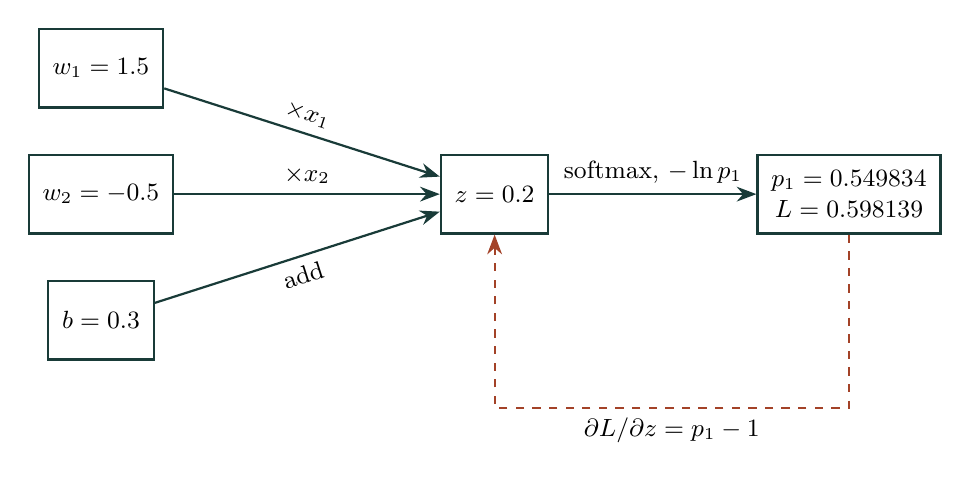
\begin{tikzpicture}[font=\small]
\node[block] (w1) at (0,1.6) {$w_1=1.5$};
\node[block] (w2) at (0,0) {$w_2=-0.5$};
\node[block] (b) at (0,-1.6) {$b=0.3$};
\node[block] (z) at (5,0) {$z=0.2$};
\node[block] (l) at (9.5,0) {$p_1=0.549834$\\$L=0.598139$};
\draw[flow] (w1)--node[above,sloped]{$\times x_1$}(z);
\draw[flow] (w2)--node[above]{$\times x_2$}(z);
\draw[flow] (b)--node[below,sloped]{add}(z);
\draw[flow] (z)--node[above]{softmax, $-\ln p_1$}(l);
\draw[grad] (l.south)--++(0,-2.2)-|node[pos=.25,below]{$\partial L/\partial z=p_1-1$}(z.south);
\end{tikzpicture}
\end{center}
$\partial L/\partial w_1$ is a \textbf{partial derivative}: how sensitively loss changes with a small change in $w_1$, holding the other independent parameters fixed. The curved $\partial$ is not a variable. The chain rule multiplies sensitivities along a computational path:
\begin{align*}
\frac{\partial L}{\partial z}&=p_1-1=-0.450166,\\
\frac{\partial L}{\partial w_1}&=\frac{\partial L}{\partial z}\frac{\partial z}{\partial w_1}
=(-0.450166)(0.2)=-0.0900332,\\
\frac{\partial L}{\partial w_2}&=(-0.450166)(0.8)=-0.360133,\\
\frac{\partial L}{\partial b}&=(-0.450166)(1)=-0.450166.
\end{align*}
Bias receives a gradient too: adding $b$ makes $\partial z/\partial b=1$. A negative derivative means a sufficiently small increase in that parameter decreases this example's loss locally.

\subsection*{One illustrative gradient-descent step}
For plain gradient descent, $\theta_{\rm new}=\theta-\eta\,\partial L/\partial\theta$. $\theta$ (``theta'') stands for any parameter; $\eta$ (``eta'') is the learning rate. With $\eta=0.1$:
\[
w_1'=1.5090033,\quad w_2'=-0.4639867,\quad b'=0.3450166.
\]
The new logit is about $0.275628$, so this example's sidewalk probability rises. Primes here mean updated values, not derivatives. \textbf{5.C uses AdamW, not this plain gradient-descent rule}. The next pages show its actual gradients, clipping, and update rule.

\guidepage{19. Backpropagation}{How error at the mask reaches millions of weights.}
\subsection*{Mathematics view}
For a known pixel, weighted focal's logit gradient is the CE gradient times $q(p_t)$:
\[
\frac{\partial\ell_n}{\partial z_{n,i,c}}
=\frac{a_{n,i}}{D_n}q(p_t)\left(p_{n,i,c}-\mathbf{1}[c=y_{n,i}]\right),
\quad D_n=\sum_i a_{n,i},
\]
\[
q(p_t)=(1-p_t)^\gamma-\gamma p_t(1-p_t)^{\gamma-1}\ln p_t.
\]
$\mathbf{1}$ is 1 when true, otherwise 0. Multiply by $1/|S|$ for a strong image or $0.5/|W|$ for a weak one. At $\gamma=0$, $q=1$: the earlier CE example. Below the numerical floor, code differentiates the clamped factor instead. Optional Dice adds its own reviewed-pixel derivatives.

If the true class is sidewalk and sidewalk probability is too low, its logit derivative is negative. A small negative-gradient step tends to increase that logit. If the true class is background and sidewalk probability is high, the derivative instead pushes the sidewalk score down.

For a parameter $\theta_j$, the chain rule connects that pixel error to earlier operations:
\[
\frac{\partial L}{\partial\theta_j}
=\sum_{n,i,c}\frac{\partial L}{\partial z_{n,i,c}}\frac{\partial z_{n,i,c}}{\partial\theta_j}.
\]
Every path using that parameter contributes. Convolutional weight sharing means many positions contribute to the same kernel's gradient. At a residual addition, the incoming gradient flows into both branches; at concatenation, it splits into the corresponding channel slices. Bilinear resize redistributes gradients using its interpolation weights.

\subsection*{Computer science view}
\code{loss.backward()} traverses PyTorch's computation graph and accumulates derivatives in each parameter's \code{.grad}. It does \textbf{not} change the parameter values. \code{optimizer.step()} changes the weights later. \code{zero_grad(set_to_none=True)} clears the previous step's gradients so they are not accidentally accumulated.

During training, intermediate activations must be retained or recoverable for backward. This is a major reason training uses more memory than inference.

\subsection*{Guardrails before the update}
The trainer checks finite losses and gradients and clips the combined gradient's Euclidean norm:
\[
g'=g\min\!\left(1,\frac{1}{\lVert g\rVert_2+10^{-6}}\right).
\]
Here $g$ collects all parameter gradients and $\lVert g\rVert_2=\sqrt{\sum_j g_j^2}$ is its Euclidean length. The maximum norm is 1, with a small denominator stabilizer. Clipping rescales the \textbf{whole gradient vector}, not each derivative separately into $[-1,1]$.

\note{Ignored pixels have zero direct supervised loss. Their surrounding image content can still influence predictions at known pixels through convolutions and normalization. ``Ignored'' does not mean the input image is erased there.}

\guidepage{20. AdamW updates}{A worked example of a weight changing.}
\subsection*{The optimizer's state}
Let $g_t$ be the gradient after clipping. AdamW keeps a moving mean $m_t$ and moving squared-gradient mean $v_t$ for every parameter:
\begin{align*}
m_t&=\beta_1m_{t-1}+(1-\beta_1)g_t,\\
v_t&=\beta_2v_{t-1}+(1-\beta_2)g_t^2,\\
\widehat m_t&=\frac{m_t}{1-\beta_1^t},\qquad
\widehat v_t=\frac{v_t}{1-\beta_2^t},\\
\theta_t&=(1-\eta_t\lambda)\theta_{t-1}
-\eta_t\frac{\widehat m_t}{\sqrt{\widehat v_t}+\epsilon}.
\end{align*}
Operations are elementwise except the earlier global clipping. The defaults are $\beta_1=0.9$, $\beta_2=0.999$, $\epsilon=10^{-8}$, and weight decay $\lambda=10^{-4}$. Bias correction compensates for moment arrays starting at zero. Decoupled weight decay shrinks parameters separately from the loss gradient. [R5, R6]

The encoder starts at learning rate $10^{-4}$ and decoder at $10^{-3}$. Both use the same decay. There are no special bias/norm decay exclusions in the current optimizer groups.

\subsection*{One pixel, one scalar weight}
This is a \textbf{cross-entropy teaching example} ($\gamma=0$), not the full focal objective. Let input $x=2$, parameter $w=0.5$, logits $(z_0,z_1)=(0,wx)=(0,1)$, and target sidewalk:
\begin{align*}
p_1&=\frac{e^1}{1+e^1}\approx0.731059,\\
L&=-\ln(p_1)\approx0.313262,\\
\frac{\partial L}{\partial w}&=x(p_1-1)\approx-0.537883.
\end{align*}
Clipping leaves this gradient unchanged because its magnitude is below 1. On the first AdamW step, $\widehat m=g$ and $\widehat v=g^2$. Using decoder learning rate 0.001:
\begin{align*}
w_{\mathrm{new}}&=0.5(1-0.001\times0.0001)
-0.001\frac{-0.537883}{0.537883+10^{-8}}\\
&\approx0.50099995.
\end{align*}
The weight increases, raising the sidewalk logit for this example. The captured FP32 execution gives approximately \textbf{0.50099993}; slight differences in the last digits are rounding, not a different rule.

\note{AdamW is not simply ``subtract learning rate times gradient.'' Its history and per-parameter normalization change the step. A real batch has many competing errors, so one update need not improve every individual image.}

\guidepage{21. Read AdamW's symbols}{Optimizer history is separate from model weights.}
\begin{tabularx}{\linewidth}{@{}lY@{}}\toprule
\textbf{Symbol} & \textbf{Read it as}\\\midrule
$\theta_{t-1},\theta_t$ & A parameter before and after update $t$. It can be a kernel entry, bias, normalization scale, or layer scale.\\
$t$ & Optimizer step count, starting at 1 here; not image number or epoch number.\\
$g_t$ & That parameter's current loss derivative, after global gradient clipping.\\
$m_t$ & Exponentially averaged gradient: a signed direction history.\\
$v_t$ & Exponentially averaged squared gradient: a magnitude history, not the variance used by LayerNorm.\\
$\beta_1,\beta_2$ & ``Beta one, beta two'': retention factors. Defaults 0.9 and 0.999.\\
$\widehat m_t,\widehat v_t$ & ``m hat, v hat'': startup-corrected moment estimates. A hat marks an adjusted quantity.\\
$\eta_t$ & ``Eta t'': the learning rate at this step. It scales the adaptive step and decay.\\
$\lambda$ & ``Lambda'': weight-decay coefficient, $10^{-4}$.\\
$\epsilon$ & ``Epsilon'': positive denominator stabilizer, $10^{-8}$ here. It is not the same constant as either normalization epsilon.\\\bottomrule
\end{tabularx}

\subsection*{What does a moving average actually do?}
For $\beta_1=0.9$, $m_t=0.9m_{t-1}+0.1g_t$: retain 90\% of the previous estimate and add 10\% of the current gradient. The squared-gradient average uses $0.999v_{t-1}+0.001g_t^2$. Squaring removes the sign; $v_t$ tracks magnitude rather than direction.

\subsection*{Why the hats?}
Both arrays start at zero. On step 1, $m_1=0.1g_1$ and $v_1=0.001g_1^2$. Dividing by $1-0.9^1$ and $1-0.999^1$ gives $\widehat m_1=g_1$, $\widehat v_1=g_1^2$. In $\beta_1^t$, $t$ is an exponent; in $m_t$, $t$ is an index. \textbf{Bias correction here is a statistical startup correction, not a learned neuron bias.}

\subsection*{Which values survive normal inference?}
The model needs $\theta$, including its learned biases. It does not need AdamW's $m,v$, gradients, learning-rate schedule, or training targets to predict a mask. Those extra arrays are saved to \emph{resume training}. Momentum-like history is optimizer memory, not memory of previous video frames in this model.

\note{The worked scalar update on the previous page uses actual AdamW. The earlier two-input example used plain gradient descent solely to show signs and the chain rule. Their different step sizes are not a discrepancy in the trainer.}

\guidepage{22. The training program}{The outer loop coordinates many small updates.}
\subsection*{Computer science view}
The following is explanatory pseudocode matching the main sequence. The real trainer also validates data, handles failures, writes files, and logs metrics.
\begin{lstlisting}
model = make_model(weights="imagenet").to(device).float()
optimizer = AdamW([
    {"params": model.backbone.parameters(), "lr": 1e-4},
    {"params": model.classifier.parameters(), "lr": 1e-3},
], weight_decay=1e-4)
scheduler = CosineAnnealingLR(optimizer, T_max=20)
objective = ReviewedFocalLoss(gamma=1.5)  # Dice off

for epoch in range(20):
    model.train()                    # stochastic depth ON
    sampler.epoch = epoch
    for images, targets, strong in training_batches:
        optimizer.zero_grad(set_to_none=True)
        logits = model(images)["out"]  # FP32 forward
        loss = objective(logits, targets, strong)[0]
        require_finite(loss)
        loss.backward()             # compute gradients
        clip_grad_norm_(model.parameters(), 1.0)
        require_finite_gradients(model)
        optimizer.step()            # change parameters
    metrics = validate(model)       # no weight updates
    scheduler.step()                # once per epoch
    save_last_and_maybe_best(metrics)
    if five_epochs_without_better_sidewalk_iou:
        break
\end{lstlisting}
\subsection*{Learning-rate schedule}
With initial rate $\eta_0$, the rate used at zero-indexed epoch $e$ is
\[
\eta(e)=\frac{\eta_0}{2}\left(1+\cos\frac{\pi e}{20}\right).
\]
At $e=0$ it is the initial rate; at $e=10$ it is half. The scheduler reaches zero after the twentieth epoch; that value is for a next epoch that is not run. There is no warmup or cosine restart in this configuration. [C3, R7]

\subsection*{Validation is a different phase}
After each epoch, binary validation references supply the checkpoint-selection metrics; partial references also supply known-sidewalk recall. Neither updates weights. A strict improvement in \textbf{sidewalk IoU} selects \code{best.pt}; otherwise the stale-epoch count increases. Training stops after five consecutive non-improving epochs or the 20-epoch limit. The loop does not automatically evaluate the held-out test partition.

{\small The base trainer retains a GradScaler interface, but it is disabled for 5.C. The pseudocode shows the equivalent ordinary FP32 operations rather than implying mixed precision is active.}

\guidepage{23. State and reproducibility}{A model file is more than a model name.}
\subsection*{Checkpoints}
\code{best.pt} contains the best validation-IoU state; \code{last.pt} contains the latest saved epoch state. Atomic writes reduce the risk of leaving a partially replaced checkpoint if the process is interrupted.

\begin{tabularx}{\linewidth}{@{}lY@{}}\toprule
\textbf{Saved item} & \textbf{Why it matters}\\\midrule
Model state & Learned encoder and decoder parameter tensors\\
Configuration & Architecture, input size, precision, initialization\\
Optimizer state & AdamW moments, update counters, parameter groups\\
Scheduler state & Where the learning-rate schedule has reached\\
Epoch / history & Progress, best IoU, stale count, logged results\\
Dataset identities & Hashes tying the run to its data and split\\
Scaler state & Disabled in FP32; not evidence of active AMP\\\bottomrule
\end{tabularx}

To resume training properly, restore the optimizer and scheduler as well as weights. Reloading only weights and starting fresh AdamW is a new optimization run, not an exact continuation.

\subsection*{What resuming can and cannot do}
The current resume path continues from the last \textbf{completed, saved epoch}, not the precise interrupted image or batch. Dataset/configuration checks protect against silently changing the experiment. The sampler is seeded by epoch. A seed helps reproducibility but does not guarantee bitwise-identical behavior across GPU types, PyTorch versions, or all execution settings.

Keep source version, environment versions, data hashes, class policy, random seeds, and the actual configuration with the run. A filename such as \code{5.C} alone cannot identify these choices.

\subsection*{Local records and W\&B}
Local history, validation reports, status files, and checkpoints remain the primary run artifacts. W\&B is a live view of metrics and approved metadata; it is not the optimizer and does not perform learning. A disconnected dashboard is not by itself proof that training stopped.

The established telemetry scope is losses, validation metrics, hyperparameters, split/dataset identities, and machine statistics. It excludes photos, masks, source code, and checkpoints. Obtain the appropriate full-run authorization before starting uploads; this document build uploads nothing to W\&B.

\note{An offline record should distinguish ``experiment completed,'' ``smoke test completed,'' ``interrupted,'' and ``not started.'' Never promote the two-update setup smoke test into evidence of trained accuracy.}

\guidepage{24. A normal prediction}{Same weights, no loss, no backward, no optimizer.}
\subsection*{The runtime sequence}
\begin{enumerate}
\item Load the matching architecture and checkpoint; validate configuration and FP32 tensors.
\item Call \code{model.eval()} and enter \code{torch.inference_mode()}.
\item Convert the camera/image input to RGB, resize, normalize, and make a batch of one.
\item Run encoder, decoder, and the two-channel output.
\item If needed, resize logits to the original image dimensions.
\item Take the winning class at each pixel and save or use the class-ID mask.
\end{enumerate}
\begin{lstlisting}
model.eval()                        # stochastic depth OFF
with torch.inference_mode():        # no autograd graph
    x = preprocess_rgb(frame).unsqueeze(0).to(device)
    logits = model(x)["out"]        # [1, 2, 540, 960]
    logits = interpolate(
        logits, size=(original_height, original_width),
        mode="bilinear", align_corners=False)
    mask = logits.argmax(dim=1)[0].to(torch.uint8)
\end{lstlisting}
This is an inference pattern, not a complete runnable loader. Use the repository's checkpoint validation and preprocessing helpers rather than inventing different normalization.

\subsection*{Mathematics view}
\[
\widehat y_i=\underset{c\in\{0,1\}}{\arg\max}\ z_{i,c}.
\]
Softmax does not change the winner, so it is optional when only class IDs are needed. For a probability display,
\[
p_{i,1}=\frac{1}{1+\exp\!\bigl(-(z_{i,1}-z_{i,0})\bigr)}.
\]
The default rule selects the greater logit; it is not a special conservative threshold tuned to eliminate flooding. With two classes, exact ties resolve to the first index in \code{argmax}, background. Softmax scores are not automatically calibrated probabilities of correctness.

\subsection*{What does not happen}
There are no targets, supervised losses, gradient calculations, or optimizer updates. Repeated drives do not improve the model unless their data is later labeled and used in a separate training process. \code{eval()} changes module behavior but alone does not disable autograd; \code{inference_mode()} handles that.

\note{The classifier predicts pixels, not centimeters, degrees, steering, or throttle. Camera geometry, IMU/encoder measurements, planning, and safety control are separate downstream systems. The model currently has no temporal memory between frames.}

\guidepage{25. Measuring performance}{Accuracy is measured against a reference, not a confidence score.}
\subsection*{Count pixel outcomes}
On \textbf{known reference pixels} only, treat sidewalk as positive: TP is correct sidewalk, FP is background predicted sidewalk, FN is missed sidewalk, and TN is correct background.
\begin{align*}
P&=\frac{\mathrm{TP}}{\mathrm{TP}+\mathrm{FP}},&
R&=\frac{\mathrm{TP}}{\mathrm{TP}+\mathrm{FN}},\\
F_1&=\frac{2\mathrm{TP}}{2\mathrm{TP}+\mathrm{FP}+\mathrm{FN}},&
\mathrm{IoU}_s&=\frac{\mathrm{TP}}{\mathrm{TP}+\mathrm{FP}+\mathrm{FN}},\\
\mathrm{IoU}_b&=\frac{\mathrm{TN}}{\mathrm{TN}+\mathrm{FP}+\mathrm{FN}},&
\mathrm{mIoU}&=\frac{\mathrm{IoU}_s+\mathrm{IoU}_b}{2}.
\end{align*}
The mIoU expression assumes both class unions are nonzero. If a class has no union, its IoU is undefined and must be handled explicitly; do not fabricate a perfect score. The same care is required for other zero denominators.

\subsection*{Interpret the metrics together}
\begin{itemize}
\item \textbf{Precision} decreases when the mask floods into known background.
\item \textbf{Recall} decreases when real sidewalk is omitted.
\item \textbf{F1} balances precision and recall but is not a boundary-distance measure.
\item \textbf{Sidewalk IoU} compares overlap with the union of the predicted and reference sidewalk.
\item \textbf{mIoU} averages sidewalk and background IoU, rather than allowing one large class to dominate pixel accuracy.
\end{itemize}
For example, $\mathrm{TP}=90$, $\mathrm{FP}=10$, $\mathrm{FN}=5$, and $\mathrm{TN}=95$ give precision 90.00\%, recall 94.74\%, F1 92.31\%, sidewalk IoU 85.71\%, background IoU 86.36\%, and mIoU 86.04\%.

\subsection*{Computer science view}
For dataset metrics, sum confusion counts over the evaluated images and then calculate the metric. That is generally different from averaging every image's metric equally. Record which aggregation you report. Native-resolution references are compared against logits resized before taking class IDs. [C3]

The current trainer exposes precision, recall, F1, and the class IoUs; the comparison viewer derives mIoU. Best-checkpoint selection currently uses sidewalk IoU, not mIoU.

\note{A positive-only reference cannot establish false positives or verified background IoU. Its known-sidewalk recall is usable, but assigning all unmarked pixels to background creates an \textbf{assumption}, not ground truth. Some existing viewer comparisons use such provisional references; keep them separate from verified binary metrics.}

{\small Segmentation IoU does not measure sidewalk width or slope error. End-to-end physical accuracy still requires matched reference measurements, calibration, and separate MAE/RMSE analysis.}

\guidepage{26. Why this architecture?}{What changed from 5.A and 5.B, and what is still unproven.}
\subsection*{The naming confusion resolved}
\begin{tabularx}{\linewidth}{@{}YYY@{}}\toprule
\textbf{Role} & \textbf{5.A / 5.B} & \textbf{5.C}\\\midrule
Encoder & MobileNetV3-Large & ConvNeXt-Tiny\\
Segmentation head & LR-ASPP & Custom U-Net-style decoder\\
Parameters & 3,218,308 & 28,855,298\\
Recorded training precision & BF16 mixed precision & Full FP32 contract\\
Floating checkpoint weights & FP32 & FP32\\\bottomrule
\end{tabularx}

MobileNetV3 is an efficiency-oriented convolutional encoder using mobile-friendly blocks. LR-ASPP is its lightweight segmentation head. Neither is another name for U-Net or ConvNeXt. Historical 5.A/5.B artifacts remain their original architecture; this guide does not rename them. [R8]

\subsection*{Why Tiny and U-Net-style fusion?}
ConvNeXt-Tiny is the smallest standard ConvNeXt variant in the referenced family. It offers more representation capacity than the existing lightweight baseline while keeping the experiment smaller than larger ConvNeXt variants. ``Tiny'' still means millions of parameters.

The decoder combines deeper semantic context with finer encoder features, a reasonable design for sidewalk boundaries. This is an engineering rationale to test, not evidence that it must beat the smaller model. Compare models under controlled data, input size, and evaluation conditions to isolate architecture effects.

\subsection*{Jetson feasibility needs measurement}
The input resolution, encoder, decoder, FP32 arithmetic, framework, transfers, and preprocessing all affect runtime. More workstation GPU memory does not prove the model will fit the car's timing budget. This code has not established real-time FP32 ConvNeXt performance on the Jetson Orin Nano.

Benchmark end-to-end latency and sustained throughput on the actual device, including image capture and downstream work. Report warmup, power mode, peak memory, and variation in latency. A hypothetical 50 Hz loop has only 20 ms for \textbf{the entire loop}, not 20 ms per component.

\note{5.C is the first implemented ConvNeXt-Tiny/U-Net-style beta in this checkout. A future 5.D is not yet a trained version or a guarantee that every one of 81k masks is correct. Do not sacrifice held-out data or annotation quality to reach an image-count target.}

\guidepage{27. Code and verification}{How to check this guide against the implementation.}
\subsection*{Local source map}
Paths below are relative to \path{code/ai_models_datasets/series_5/} in the repository. Trainers live here; supporting code and configs stay in \path{tools/}. Reusing A/B training code does not change the C model's architecture.

{\small
\begin{tabularx}{\linewidth}{@{}l >{\hsize=1.15\hsize}Y >{\hsize=.85\hsize}Y@{}}\toprule
\textbf{ID} & \textbf{File} & \textbf{Authority for}\\\midrule
C1 & \path{tools/models/convnext_tiny_unet.py} & Encoder, decoder, FP32 checks\\
C2 & \path{tools/configs/series_5_c_config.json} and \path{series_5_c_sidewalkpilot_trainer.py} & 5.C defaults, data-count gate, model wiring\\
C3 & \path{series_5_a_sidewalkpilot_trainer.py} & Shared data transforms, sampler, training, checkpoints, evaluation, prediction\\
C4 & \path{series_5_b_sidewalkpilot_trainer.py} & Screened batch composition and conservative loss\\
C5 & \path{tools/filtering/pseudo_mask_filter.py} and \path{tools/datasets/pseudo_training_targets.py} & Pseudo-label filtering and target preparation\\
C6 & \path{tools/models/segmentation_losses.py} & 5.C focal baseline and reviewed-only Dice\\\bottomrule
\end{tabularx}}

\subsection*{Reproducible document checks}
\code{capture_facts.py} instantiates an untrained copy on CPU, hooks feature-map outputs, and checks FP32 and parameter counts. It also runs \code{verify_teaching_examples.py}: normalization, matrix arithmetic, convolution, layer biases, GELU, softmax, and weight/bias gradients are checked against PyTorch. The loss/AdamW examples are checked too. These checks do \textbf{not} train the research model. Results go in \code{implementation-facts.json}.

Captured environment: PyTorch \textbf{2.7.1+cu118}; torchvision \textbf{0.22.1+cu118}. Source hashes in the JSON identify the audited files. The LaTeX build checks these hashes, compiles the \code{.tex} source, verifies Computer Modern fonts and pagination, and renders the PDF for inspection.

\begin{lstlisting}[language=bash]
# From this document's directory on the workstation:
/home/rsabavat/.gpu-env/bin/python capture_facts.py
/home/rsabavat/.venvs/sidewalkpilot-docs/bin/python build_latex.py

# Standalone typesetting, without the local code audit:
tectonic sidewalkpilot-5C-math-and-cs.tex
\end{lstlisting}
The \code{.tex} file is a standalone LaTeX source, also suitable for a standard LaTeX installation or Overleaf. The original Typst source is retained as an archive; this PDF uses actual LaTeX with classic Computer Modern text and mathematics.

\subsection*{Evidence boundaries}
The earlier local two-update GPU smoke run verifies basic execution and saving, not learned generalization. Mathematical examples verify formulas, not mask quality. This guide is an AI-assisted explanation checked against local source; it is not a replacement for the researcher's notebook, approved research plan, or final experimental report.

{\small Safety-critical field operation still depends on the approved supervision and control system, not on a high segmentation metric. This document makes no new claim about operating permission.}

\guidepage{28. Symbol reading desk}{A reference for the notation, not another set of model parameters.}
\begin{tabularx}{\linewidth}{@{}lY@{}}\toprule
\textbf{Notation} & \textbf{How to read it in this guide}\\\midrule
$\mu,\sigma,\sigma^2$ & Mu: mean. Sigma: standard deviation. Sigma squared: variance. Context tells you whether they are fixed reference values or statistics of current activations.\\
$\sum_{j=1}^{M}q_j$ & Add $q_1+q_2+\cdots+q_M$. $j$ is a summation index; $M$ is its upper limit.\\
$x_{c,h,w}$ & Select one tensor entry using channel, row, and column indices. Subscripts do not mean multiplication.\\
$x^2,\sqrt{x}$ & Square $x$; take its nonnegative square root (for $x\ge0$). A superscript is a power here, not an index.\\
$\theta,\eta,\lambda$ & Theta: parameter(s). Eta: learning rate. Lambda: decay strength. These are Greek letters, not special computer types.\\
$\gamma,\beta,\epsilon$ & Gamma: learned residual scale or configured focal exponent, depending on context. Beta: optimizer retention factor. Epsilon: a small stabilizing constant.\\
$\partial L/\partial\theta$ & Partial derivative of loss with respect to one parameter, holding other independent parameters fixed.\\
$\lVert g\rVert_2$ & Euclidean length of a vector: square entries, add them, take the square root.\\
$\bar u,\widehat m$ & U bar: a mean here. M hat: corrected optimizer estimate. A hat can also denote a prediction, as in $\widehat y$.\\
$\odot,\op{concat}$ & Multiply matching entries; stack arrays along a chosen axis. Neither means matrix multiplication.\\
$|S|,n\in S$ & Number of elements in a set; membership in that set. By contrast, $|g|$ for a scalar means absolute value.\\
$\lfloor r\rfloor,\lceil r\rceil$ & Floor rounds down; ceiling rounds up. For 2.3 these give 2 and 3.\\
$\arg\max_c z_c$ & Return the class index with the largest score, not the score itself.\\
$\approx,\propto$ & Approximately equal; proportional to. Neither is an exact equality sign.\\\bottomrule
\end{tabularx}

\subsection*{Symbols are local names, not universal meanings}
$W$ can mean a weight matrix, image width, or the set of weak examples; its definition in that equation decides. $b$ may name a learned bias, while a subscript $b$ on IoU names background. $e$ is Euler's number in $e^z$, but the epoch index in $\eta(e)$. In the schedule, $\pi\approx3.14159$ and cosine uses radians.

\note{Read an unfamiliar formula in this order: identify the output; name each input and its shape; read indices and summation limits; follow arithmetic operations; then ask which quantities are learned, computed from this batch, or fixed settings.}

\guidepage{29. References and vocabulary}{Primary sources; implementation takes precedence over generic examples.}
{\small
\textbf{R1.} Liu, Zhuang, et al. ``A ConvNet for the 2020s.'' 2022.
\refsource{https://arxiv.org/abs/2201.03545}{arxiv.org/abs/2201.03545}

\textbf{R2.} PyTorch / torchvision 0.22. ConvNeXt implementation.
\refsource{https://docs.pytorch.org/vision/0.22/_modules/torchvision/models/convnext.html}{Versioned ConvNeXt source}

\textbf{R3.} Ronneberger, Olaf, Philipp Fischer, and Thomas Brox. ``U-Net: Convolutional Networks for Biomedical Image Segmentation.'' 2015.
\refsource{https://arxiv.org/abs/1505.04597}{arxiv.org/abs/1505.04597}

\textbf{R4.} PyTorch v2.7.1. \code{cross_entropy} implementation and API contract.
\refsource{https://github.com/pytorch/pytorch/blob/v2.7.1/torch/nn/functional.py}{torch/nn/functional.py}

\textbf{R5.} PyTorch v2.7.1. AdamW implementation; inherited update implementation in Adam.
\refsource{https://github.com/pytorch/pytorch/blob/v2.7.1/torch/optim/adamw.py}{adamw.py} and
\refsource{https://github.com/pytorch/pytorch/blob/v2.7.1/torch/optim/adam.py}{adam.py}

\textbf{R6.} Loshchilov, Ilya, and Frank Hutter. ``Decoupled Weight Decay Regularization.'' 2017; ICLR 2019.
\refsource{https://arxiv.org/abs/1711.05101}{arxiv.org/abs/1711.05101}

\textbf{R7.} PyTorch v2.7.1. \code{CosineAnnealingLR} implementation.
\refsource{https://github.com/pytorch/pytorch/blob/v2.7.1/torch/optim/lr_scheduler.py}{torch/optim/lr\_scheduler.py}

\textbf{R8.} Howard, Andrew, et al. ``Searching for MobileNetV3.'' 2019.
\refsource{https://arxiv.org/abs/1905.02244}{arxiv.org/abs/1905.02244}

\textbf{R9.} Torchvision 0.22. \code{Normalize}: channel-wise mean and standard deviation.
\refsource{https://docs.pytorch.org/vision/0.22/generated/torchvision.transforms.Normalize.html}{Versioned preprocessing documentation}

\textbf{Further reading.} Ananthaswamy, Anil. \emph{Why Machines Learn: The Elegant Math Behind Modern AI}. Dutton, 2024.
\refsource{https://www.penguinrandomhouse.com/books/677608/why-machines-learn-by-anil-ananthaswamy/}{Publisher's book page}. Suggested for mathematical intuition; the examples and diagrams in this guide are original, not reproductions of the book.
}
\subsection*{Compact vocabulary}
{\small
\begin{tabularx}{\linewidth}{@{}lY@{}}\toprule
\textbf{Encoder} & Transforms pixels into progressively coarser, richer features.\\
\textbf{Decoder} & Combines and enlarges features to make spatial predictions.\\
\textbf{Logit} & A class score before softmax; may be negative or positive.\\
\textbf{Parameter} & A number learned by the optimizer, such as a kernel weight.\\
\textbf{Hyperparameter} & A configured choice, such as learning rate or batch size.\\
\textbf{Gradient} & A local derivative describing how loss changes with a parameter.\\
\textbf{Batch / step} & A group of examples / one optimizer update using that group.\\
\textbf{Epoch} & One traversal defined by the sampler, possibly with repeats.\\
\textbf{Inference} & Applying existing weights without training updates.\\
\textbf{Pseudo-label} & A generated training target whose correctness is not guaranteed.\\\bottomrule
\end{tabularx}}

{\small Expanded teaching edition: 22 November 2026. Links identify papers and versioned documentation; local hashes preserve which project code this document describes.}
\end{document}
